%%for NRA TODO: edit/rewrite as follows:
%%(i) assurance argument: what specifically is the assurance signal? as opposed to value alignment, the signal here is some visualization or access to the decision-making process itself...the user is not just looking at the end result or utility of the AIA decision making process, or at behaviors that try to align the AIA's behavior/utility with the user's intent frame. Rather, the user gets some form of access to dig deeper into the AIA behavior to see what informs the utility function, or more generally the different steps along the way that generate different parts of the AIA's actual behavior (as opposed to a simplified or approximate explanation of its behavior, which is covered later)...in almost all cases, the model or intermediate model outputs are generally displayed to or accessed by users in some graphical manner, with some accompanying text/dialog/annotations...
%%(ii) what is mechanism for generating appropriate TRBs? if user gets to dig in, then they get to assess competency and predictability components of trust ; if models are interpretable, then user can in principle understand how to `do the task themselves in exactly the same way an AIA would do it' (i.e. by programatically imitating AIA's behavior on task)-- this follows a theory of mind argument, in that it should allow user to build a better `mental model' of what the AIA would consider to be `situational normality' and how AIA would handle different situations. Caveat here is that this could go south if the user mis-interprets or only understands part of what the AIA is actually doing, either in terms of interpretable model or the nature of the task itself -- this is a significant risk in highly complex or specialized problems where user may not have sufficient training or expertise. This also poses concerns for how/when user can access such models -- unlike value alignment (where user accesses assurances only through behavior of AIA itself), user has more freedom in deciding when and how to peek under the hood -- relates somewhat to problem of information visualization discussed later, except that here the information being given to the user are the actual AIA algorithms, as opposed to by products or after effects of those capabilities
%%(iii) how can designers build/exploit interpretable models for AIAs, i.e. what techniques available for interpretable model building? This gets to summarizing what Brett has written below -- can keep papers clustered more/less as they are, but need to repeat the assurance arguments above: 
%%(a) assessment of interp: post hoc approaches that map models to domain knowledge, place constraints on model inputs, or examine handling of known nonlinear effects;  
%%(b) creating interpretable models: compress this section into key ideas with citations of relevant papers/methods: model could be interpretable from outset like a decision tree (at the expense of performance), or could be less interpretable from outset and then post-fit with another interpretable model. Important thing to note is that most of these are designed around machine learning and pattern recognition problems -- and as such require that the tasks being performed by the AIA to be mappable to these kinds of problems; this generally means that some form of training data is required for supervised or unsupervised learning. ALSO: second approach of building a more interpretable model around an intial model technically counts as a `supplementary' method, in that this interpretable -- DOES THIS ALREADY COME LATER IN SURVEY???
%%(c) human-in-loop learning -- very similar to value alignment, except that not necessarily only concerned with learning utility, but also other kinds of features or useful tidbits that aid in AIA decision making -- follows same theory of mind argument from before: user will have same mental grounding as AIA, so trust can be calibrated appropriately to get better understanding of predictability, competence, and situation normality...Julie Shah's work on learning LTL rules from data?? can maybe leave (c) out for time being....
\subsection{Interpretable Models and Processes} \label{sec:interp_models}
%%\nisarcomm{add `processes' to label of this category...}
Another way to provide assurances about AIA conformance to user intent frames is to expose the models and algorithmic processes governing its actions directly to the user. If these models and processes also happen to be easy for users to interpret, then the user can (ideally) acquire a well-formed and highly predictive `theory of mind' for the AIA's behavior, with little or no effort . 
\citet{Doshi-Velez2017-xy} give an argument for why interpretability is critical in AIA systems since interpretability `is used to confirm other important desiderata of [machine learning] systems'. 
Yet, perhaps unsurprisingly, `interpretability' and the attendant desiderata still elude formal universally accepted definitions. 
%%Based on our survey, and building on the `easily accessible theory of mind' notion: we define an interpretable model or process here as one which can be fully comprehended by a typical human user, to the degree that the user herself could (given access to the model/process, and enough time and resources for performing required intermediate computations) precisely predict the results that an AIA would obtain on a given task. In other words: a model or process made so easy to understand that a human could do it. \nisarcomm{need to think carefully about implications of this definition: in principle any human could execute any algorithm given enough time/computation, so this isn't saying much...something else needed here to refine this idea...}. 
They also use the words `interpretable' and `explainable' interchangeably. In contrast, we treat them as distinct descriptors. We discuss models that are inherently interpretable here, and models that can be understood by explanation in Section~\ref{sec:reduce_complexity}.  The difference is that interpretability (in our view) implies that the actual process/model used by an AIA is self-explanatory, whereas explainable models can be made interpretable by post hoc operations but do not necessarily explain the actual model/process used by an AIA. 
Being able to interpret the actual model/process used by an AIA helps human users to more appropriately understand their behaviors, and thus exhibit appropriate TRBs in turn. This approach to assurance also captures broader AIA processes and models that rely on rules, heuristics, etc., rather than just those that rely on optimization of some particular utility. 
%%\nisarcomm{need to unpack this still further -- see tex comments above }

\subsubsection{Common Approaches:}
Two main approaches to designing interpretable AIA models and processes are considered here. 
The first is to \emph{assess an existing set of candidate models/processes} in order to evaluate their interpretability in the context of a particular task, and then select the best candidate. 
This is typically done with certain classes of models or solution processes, e.g. whether to use decision trees vs. decision tables for a given planning task. 
The second is to \emph{synthesize interpretable models/processes} by leveraging human designer input during the model/solution-building process. 
The first approach requires pre-defined measures of interpretability, and thus some mechanism for capturing ability to gain insights into competence, predictability, and situation normality. This also presupposes that the model/process candidates are inherently interpretable along these lines to begin with, which may rule out certain model/process families that perform well on certain tasks. 
The second approach allows designers to apply domain knowledge to determine metrics for interpretability, although this can lead to solutions that do not perform as well as those that are less interpretable. 
%%\nisarcomm{where and hwo do (intrinsic) assurances fall out of these?}

What is the assurance mechanism that potentially leads to proper TRBs in either approach? 
Essentially, allowing the user to access and examine an interpretable model/process also allows them to simultaneously assess competency, predictability, and situational normality components of trust. If the models/proceses are interpretable, then a user would understand exactly how the AIA would perform its task (i.e. down to a mechanical/programmatic level). 
This gives the user a `mental model' of what the AIA would consider to be situational normality and how AIA would respond in different situations (predictability and competence). 
The caveat here is that incorrect TRBs may arise if the user mis-interprets or only understands part of the model/process. 
This is a significant risk in highly complex or specialized problems, where users may not actually have sufficient training or expertise. This also poses concerns for how/when user can access interpretable AIA components. 
Unlike value alignment (where user accesses assurances only through behavior of AIA itself), the user has more freedom in deciding when and how to `peek under the hood'. This relates to assurances based on information visualization discussed later, except that here the information being given to the user are the actual AIA algorithms themselves, as opposed to by products or after effects of those algorithms. %%\nisarcomm{I need to trim this down a bit?}

\paragraph{Assessing Interpretability:}
\citet{Van_Belle2013-ph} suggested three ways to ascertain the level of interpretability and potential utility of learned models (compare to categories proposed by \citet{Lipton2016-ug}): 1) Map them to domain knowledge; 2) Ensure safe operation across the full operational range of model inputs; and 3) Assess whether important non-linear effects are accurately accounted for. This work identifies certain strengths and weaknesses of different techniques, but ultimately concludes that no method is clearly best in all situations. 
%%%\nisarcomm{need to say a little bit more about the actual methods proposed -- how does one, for instance, go about doing 1 or 2 or 3? don't need to give specific details, but mention what techniques available}
%
Along similar lines, \citet{Huysmans2011-th} compared decision trees, decision tables, propositional if-then rules, and oblique rule sets to understand which set of methods is `most interpretable'. It was experimentally determined that decision trees and tables tend to be easier to interpret, but it is noted that each method could perform better than others in different applications. For example decision trees and tables are typically better suited for answering a symbolic question (which requires a local understanding of a model) like: \emph{how does the model classify observation $X$'?}. This is in contrast to a spatial question (which requires a global understanding of the model) like: \emph{is it correct that applicants with a high income are more likely to be accepted than applicants with a low income?}
%
Having quantified the interpretability of a model given different classes of problems, and different requirements of users the appropriate model can then be selected during design to fit the needs of a specific application.

\paragraph{Interpretable Model Synthesis:}
\citet{Ruping2006-xj} asks how classification results and the accuracy-interpretability trade-off can be made more transparent to those who design and use classifiers. He explores one approach by combining simpler global models with more complex local models that are built around learning results (\citet{Otte2013-oo} and \citet{Ribeiro2016-uc} implement similar ideas as well). 
Figure \ref{fig:ruping} illustrates this idea. 
The explanation of Fig.~\ref{fig:ruping} could be something like: `The classification boundary is generally a horizontal line. However, for a small region on the right hand side the boundary is shaped roughly quadratic starting from the horizontal line'.
%\brettcomm{The explanation of Fig.~\ref{fig:ruping} could be something like: `The classification boundary is generally a horizontal line. However, for a small region on the right hand side the boundary is shaped roughly like a square root starting from the horizontal line'.---I like the example of \emph{how} global/local could be used}

%%%%%%%%%%%%%%%%%%%%%%%%%
\begin{figure}[htbp]
    \centering
    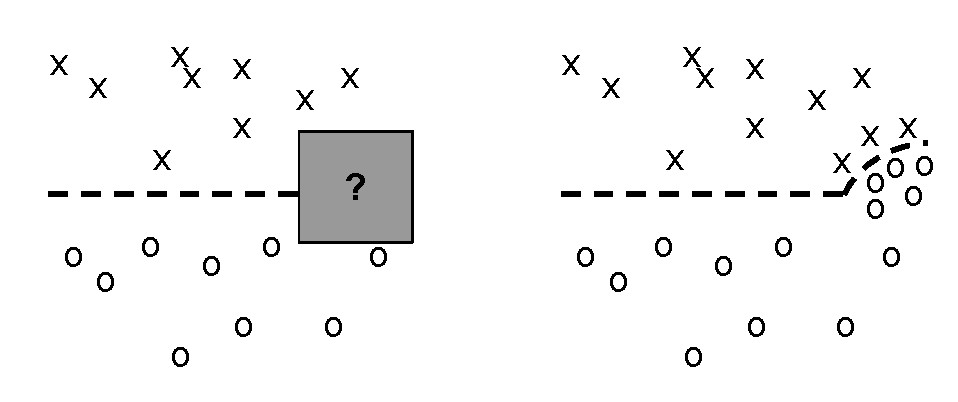
\includegraphics[width=0.5\textwidth]{Figures/global_local}
    \caption{Example of simple global interpretable learning model on the left, and on the right a more complex locally interpretable learning model that can be used when more precise understanding of a specific decision made by the learner is required. }
    \label{fig:ruping}
\end{figure}
%%%%%%%%%%%%%%%%%%%%%%%%%

Considerable effort has also gone into endowing `grey box' and `black box' models with interpretable features. 
For instance, \citet{Abdollahi2016-vn} investigate making collaborative filtering models more interpretable by using a conditional restricted Boltzmann machine (RBM). \citet{Ridgeway1998-lv} use `weight of evidence' (WoE) as a boosting method that is more amenable to interpretation, and show that the performance WoE is on par with AdaBoost. \citet{Choi2016-by} construct a recursive attention neural network to remove recurrence on the hidden state vector, and instead add recurrence on the visits of patients to doctors, as well as on different diagnoses during those visits. In this way the model is able to predict possible diagnoses in time, and a visualization can be that that indicates the critical visits and diagnoses that lead to that prediction.

Learning of human-understandable representations for data and feature selection also provides another avenue for developing assurances  \cite{Bengio2013-uv, Guyon2003-fj}. For instance, \citet{Mikolov2013-lt} studied how to represent words and phrases in a vector space for natural language text learning; this enables simple vector operations for understanding word sense similarity and relative relationships learned from text corpora. For example, the vector addition operation \emph{airlines+German} yields similar entries that include \emph{Lufthansa}. Such representations encode knowledge that can be easily checked and understood by humans, and thus implicitly facilitate interaction and calibration of trust (see \cite{Haury2011-zi} for another example). The problem of discovering human understandable features and representations in more general settings still remains an open question. Currently, the main question for representation learning is how to find the `best representations' for a particular application---not necessarily the representations and features that are `most humanly understandable'. This is not surprising, since human-understandable representations and features are not necessarily optimal for the criteria that AIAs are typically designed against. 

Contrary to the belief that interpretable models are necessarily worse performing than their less interpretable counterparts, several researchers have shown that this is not always the case (at least in the context of machine learning). However, the real trade-off is the amount of work that goes in to crafting the interpretable model from the start; these methods are often custom designed for certain tasks and are not easily transferable to other problems. Because of this, AIA designers must strike a balance between \emph{interpretable models}, \emph{explainable models}, and \emph{black-box models}.

\citet{Park2016-ld} point out that real interpretability in complex tasks still requires expert knowledge to make sense of complicated features; in essence: \emph{people are needed at both ends of interpretable models}. For instance, \citet{Jovanovic2016-gw} use `Tree-Lasso' (TL) logistic regression with domain knowledge (i.e. medical diagnostic codes) to group similar conditions, and then use TL regression again on that information to develop a sparser model. \citet{Zycinski2012-jj} also use domain knowledge to structure a data matrix before feature selection and classification. See also \citet{Zhang2018-no,Khoa2018-gh} for other related examples. 
%
This kind of approach is also illustrated by those who use those who use `theory guided data science' (TGDS~\cite{Kumar2016-yw,Faghmous2014-og}). As one example \citet{Morrison2016-fz} address the situation where an imperfect analytical model is available for chemical reaction kinetics: the theoretical reaction equations are well known, but a `stochastic operator' is added on top of this to account for uncertainties and modeling errors. In adopting this approach the model becomes interpretable (to experts).

\subsubsection{Grounding Example:}
In the case of the `VIP Escort' problem (described in Section~\ref{sec:mot_example}), interpretable models might be used as an assurance in the following way, starting with the assumptions that:

\begin{itemize}
    \item The UGV has just begun an attempt to escape the road-network
    \item The UGV is using a decision-tree for selecting different movements
    \item The operator is able to view the decision-tree model the UGV is using
\end{itemize}

While the operator is monitoring the progress of the UGV in its attempt to escape the road-network they are able to consult the decision-tree model. In this case the operator chose to consult the table when they saw the UGV make an unexpected turn at a given intersection. The operator identified the conditions that led to the decision and found that the UGV was not well equipped to execute the decision the operator thought was best.
\paragraph{\textbf{Discussion of Example:}} In this example the use of a decision-tree as a model enabled the operator to investigate unexpected behavior. During inspection they identified certain conditions that led to a decision, and they found that the UGV was not \emph{competent} to perform what the operator thought was a better decision. Because of this the operator better understood the decision the UGV made.
